\subsection{Sprachsynthese}

Dieses Kapitel beschreibt die Integration der Sprachsynthese in das Praxisrufsystem.
Der Fokus liegt dabei auf den Abläufen zum Empfangen von Benachrichtigungen und dem Abrufen von Sprachdaten.
Die Integration von notwendigen Schnittstellen im Mobile Client wird im Kapitel 5.2 beschrieben.

\subsubsection{Konfiguration}

Nach Use Case U03\footnote{Siehe Kapitel 3} muss der Praxismitarbeitende alle Sprachbenachrichtigungen stummschalten können.
Dazu wird der Mobile Client um eine Settings Ansicht erweitert.
Auf dieser Ansicht, kann der Benutzer auswählen, ob Benachrichtigungen vorgelesen werden sollen.
Ist die Option deaktiviert, werden Benachrichtigungen nie vorgelesen.

\begin{figure}[h]
    \centering
    \begin{minipage}[b]{0.75\textwidth}
        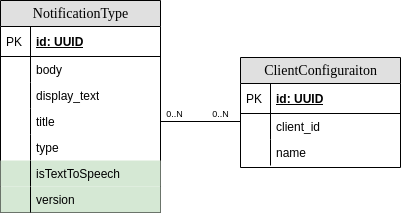
\includegraphics[width=\textwidth]{/home/joshua/FHNW/dev/IP6/IP6_Bachelorarbeit_Bericht_Cloudbasiertes_Praxisrufsystem/src/graphics/diagramms/erd_t2s_v01.drawio}
        \caption{ERD Ausschnitt - Konfiguration Sprachsynthese}
    \end{minipage}
\end{figure}

Benachrichtigungen für Praxisruf können über das Admin UI konfiguriert werden.
Es kann pro Benachrichtigung Titel, Inhalt, Anzeigetext für Benachrichtigungsbuttons und eine Beschreibung erfasst werden.
Diese Konfiguration wird über die Entität NotificationType verwaltet.
Neu soll auch konfiguriert werden können, ob eine Benachrichtigung für die Sprachsynthese relevant ist.
Dazu wird die Entität NotificationType um ein boolean Flag mit dem Namen isTextToSpeech erweitert.
Dieses Flag wird beim Versenden einer Benachrichtigung mitgesendet und kann vom Empfänger überprüft werden.
Insofern Sprachbenachrichtigungen in den Einstellungen aktiviert sind, werden Benachrichtigungen, welche dieses Flag auf TRUE gesetzt haben vorgelesen.

Neben dem Feld isTextToSpeech, wird die NotificationType Entity um ein weiteres Feld version erweitert.
Dieses Version Feld beinhaltet eine Ganzzahl welche mit jeder Änderung inkrementiert wird.
Das Version Feld wird ebenfalls beim Versenden von Benachrichtigungen mitgesendet und kann auf Client Seite zur Implementierung eines Caches verwendet werden.


\clearpage
\subsubsection{Integration Sprachsynthese Provider}

Die Anbindung des Sprachsynthese Providers erfolgt zentral im Cloudservice.
Mobile Clients sprechen den Sprachsynthese Provider nie direkt an.
Sie kommunizieren stattdessen mit dem Cloudservice, welcher Anfragen an den Sprachsynthese Provider ausführt und die Resultate an den Mobile Client weiterleitet.
Dazu wird der Cloudservice um ein Modul mit dem Namen Speech Synthesis erweitert.
Das Speech-Modul darf gleich wie die Module Configuration und Notification keine direkten Abhängigkeiten auf andere Cloud Service Module haben.
Sämtliche notwendige Kommunikation zwischen den Modulen findet über Rest-Schnittstellen statt.
Diese Unabhängigkeit ermöglicht es, das Modul in Zukunft einfach aus dem Cloudservice auszubauen und als eigenständigen Micro-Service zu betreiben.

Wie in Kapitel 4.2 beschrieben, wird AWS Polly als Sprachsynthese Provider für dieses Projekt verwendet.
Demenstprechend, muss die Anbindung im Cludservice für AWS Polly implementiert werden.
Die Abhängigkeit an einen spezifischen Provider soll dabei soweit wie möglich minimiert werden.
So kann bei Bedarf einfacher auf einen anderen Provicer gewechselt werden.
Um dies zu ermöglichen wird das Interface SpeechSynthesisService definiert.
Dieses gibt eine einzelne Methode vor, welche eine InputStreamResource zurückgibt und eine Universal Unique Id als Parameter entgegennimmt.
Der Parameter entsprocht dabei der technischen Identifikation des zu synthetisierenden Benachrichtigungstypes.
Die InputStreamResource muss die snythetisierten Sprachdaten enthalten.

\begin{figure}[h]
    \centering
    \begin{minipage}[b]{1\textwidth}
        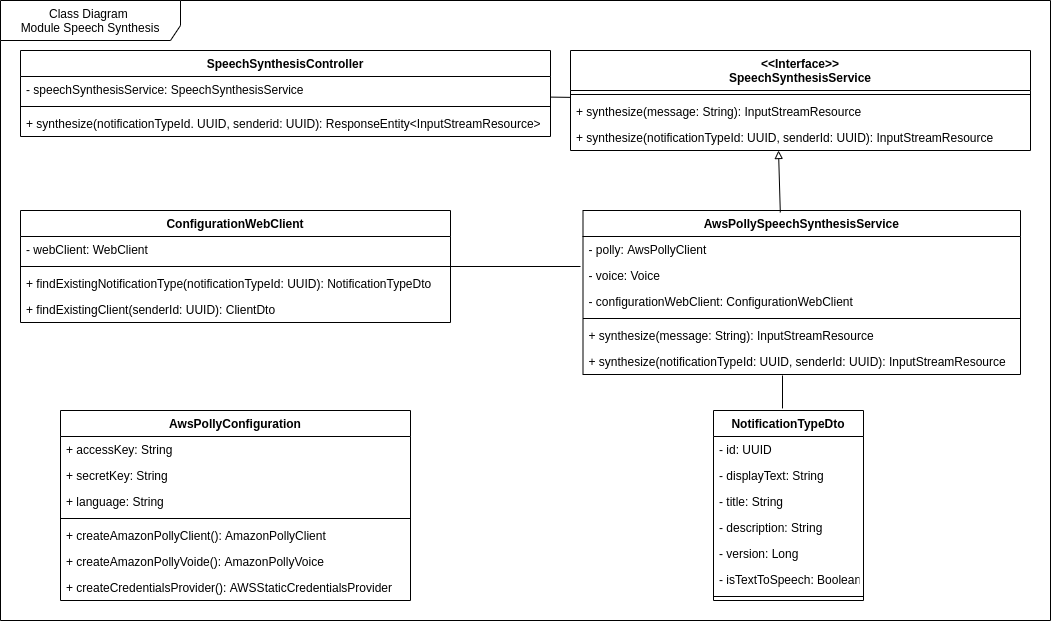
\includegraphics[width=\textwidth]{/home/joshua/FHNW/dev/IP6/IP6_Bachelorarbeit_Bericht_Cloudbasiertes_Praxisrufsystem/src/graphics/diagramms/Class_AWS_Polly_Configuration_V02}
        \caption{Klassendiagramm Modul SpeechSynthesis}
    \end{minipage}
\end{figure}

Dieses Interface kann als Abhängigkeit im Endpunkt, mit welchem Mobile Clients kommunizieren verwendet werden.
Um einen spezifischen Sprachsynthese Provider zu unterstützen, reicht es aus, dieses Interface zu implementieren und eine entsprechende Instanz zur Verfügung zu stellen.

Für dieses Projekt bedeutet dies, dass ein SprachSyntheseProviderService für AWS Polly implementiert werden.
AWS Polly bietet einen Java SDK, welcher die Anbindung ermöglicht.
Dieser SDK bietet alle Klassen die für die Anbindung an AWS Polly nötig sind und wird in der Implementierung des SprachSyntheseProviderService verwendet, um den Service anzubinden.

Konkret benötigt es für die Anbindung von AWS Polly drei Komponenten.
Als Erstes muss ein AWSStaticCredentialsProvider zu Verfügung gestellt werden.
Dieser liefert die Credentials, welche das System berechtigen, Anfragen an AWS Polly zu senden.
Als zweites muss eine Voice konfiguriert werden.
Diese definiert Sprache und Stimme, welche für die Synthetisierung der Sprachdaten verwendet wird.
Letztlich muss ein AmazonPollyClient konfiguriert werden.
Dieser Client wird verwendet, um Anfragen an AWS Polly zu senden.
Er verwendet den zuvor konfigurierten CredentialsProvider, um die Anfrage mit den entsprechenden Credentials zu ergänzen
und die konfigurierte, Voice um die Daten entsprechend zu synthetisieren.

Da im Cloudservice Spring Boot verwendet wird, können diese Komponenten in einer Spring Konfigurationsklasse konfiguriert und instanziert werden.
Im konkreten Service können diese dann als Abhängigkeiten angegeben werden und stehen über die Spring Dependency Injection zur Verfügung.
Die Properties welche für die Konfiguration notwendig sind, werden aus dem application.yml für das aktuell aktive Profil geladen.
Sprache und Region werden sich im Rahmen dieses Projektes nie ändern und beinhalten keine sensitiven Informationen.
Sie werden deshalb direkt im application.yml definiert und mit dem Quellcode des Projektes verwaltet.
Als Credentials für die Anbindung dienen die zwei Schlüssel AccessKey und SecretKey.\footnote{quote here}
Diese werden nicht direkt im application.yml abgelegt.
Für sämtliche Credentiels wird im application.yml ein Platzhalter definiert, welcher die Credentials aus entsprechend benannten Umgebunsvariablen lädt.
Die Zugangsdaten müssen damit nicht mit dem Quellcode verwaltet werden und können einfach ausgetauscht werden.
In der Implementation des Services kann nun über den injezierten AmazonPollyClient eine Abfrage an den Speech Synthesis Service gesendet werden.

\subsubsection{Schnittstelle Cloud Service}

Das Speech-Modul stellt einen Endpoint zur Verfügung über den die Sprachdaten zu einer Benachrichtigung abgefragt werden können.
Der Endpoint bietet dabei nicht die möglichkeit generische Daten in Sprachdaten zu verwandeln.
Stattdessen erlaubt er es Sprachdaten für die aktuelste Version von bekannten Benachrichtigungstypen zu beziehen.
Der einzige Parameter für diese Anfragen ist die technische Identifikation des Benachrichtigungstyps (NotificationType) der relevanten Benachrichtigung.
Anhand dieses Identifikators können die Informationen des Benachrichtigugnstyps über die REST-Schnittstelle des Configuration-Modul angefragt werden.
Dadurch können Änderungen an einem Benachrichtigungstyp direkt angewendet werden, ohne dass die Informationen auf dem Mobile Client aktualisiert werden müssen.
Die geladenen Daten können dann verwendet werden um eine Anfrage an den Sprachsynthese Provier zu senden.
Die vom Provider gelieferten Sprachdaten können anschliessend als Resultat an den Client zurügegeben werden.
Der Endpunkt für die Abfrage von Sprachdaten im Cloud Service wird als Spring RestController umgesetzt.
Die Sprachdaten werden dabei als Binärdaten mit Media Type ''audio/mp3'' im Body der Response zurückgegeben.
Auf Client Seite, kann dieser Endpunkt so als Download angesprechen werden.

\clearpage
\subsubsection{Anbindung Mobile Client}

Für die Integration des SpeechSynthesis Endpunkts aus dem CloudService muss die in Kapitel 5.2 beschriebene Klasse PraxisrufApi erweitert werden.
Neben dem Abfragen von JSON Daten über HTTP Schnittstellen, muss diese für die Sprachsynthese auch das herunterladen von Dateien unterstützten.
Dies kann URLSession aus der iOS Standardbibliothek bietet dafür mit URLSession.downloadTask die Möglichkeit Inhalte von einer URL herunterzuladen.\cite{ios_downloadtask}
Der Service PraxisrufApi wird dementsprechend um eine Methode download ergänzt.
Diese ist dafür verantwortlich, eine Anfrage für den Download mit Credentials aus dem iOS Keystore zu ergänzen und die Abfrage zu versenden
und die Resultate oder Fehler an den mitgegebenen CompletionHandler zu übergeben.\footnote{Vgl. Kapitel 5.2}
Heruntergaladene Dateien werden vom PraxisrufApi in einem temporären Verzeichnis gespeichert.
Das Resultat im Erfolgsfall ist deshalb nicht die heruntergeladene Datei selbst, sondern eine URL welche auf die Datei im temporären Verzeichnis zeigt.
Die Sprachsynthese für Benachrichtigungen, soll automatisch ausgeführt werden sobald eine relevante Benachrichtigung empfangen wurde.
Die Benachrichtigung wird im AppDelegate empfangen, aufbereitet und an die Applikation übergeben.
Die aufberetieten Daten beinhalten, die Information, ob die Benachrichtigung für die Sprachsynthese relevant ist.
Dies kann dem isTextToSpeech Flags in der Benachrichtigung entnommen werden.
Für die Verarbeitung der Sprachdaten, wird ein eigener Service erstellt.
Dieser SpeechSynthesisService verwendet die Downloadfunktion aus der PraxisrufApi Basisklasse, um Sprachdaten vom Cloudservice abzufragen.
Wurden die Daten erfolgreich geladen, kopiert er die heruntergeladenen Daten aus dem temporären Downloadverzeichnis in ein permanentes Verzeichnis.
Die Datei wird dabei unter dem Namen ''ID NotificationType''.''version'' gespeichert.
Anschliessend werden die Inhalte der Datei als Audio wiedergegeben.
Die Namenskonvention für die gespeicherten Dateien, erlaubt es ein einfaches Cache zu implementieren.
Bevor der SpeechSynthesisService eine Anfrage an den Cloudservice absetzt, prüft er, ob bereits eine Datei mit dem entsprechenden Namen vorhanden ist.
Ist dies der Fall, wird keine Anfrage versendet und die Datei wird direkt abgespielt.
Die Id des NotificationTypes im Dateinamen sorgt dafür, dass pro Benachrichtigungstyp nur einmal Sprachdaten abgefragt werden müssen.
Die Version des NotificationTypes im Dateinamen sorgt dafür, dass die Daten bei einer Änderung am Benachrichtigungstyp neu geladen werden.
Da der Inhalt einer Benachrichtigung im Cloudservice abgefüllt wird, bedeuet dies das Benachrichtigungen immer in der neusten Version angezeigt werden.
Durch die beschriebene Implementierung des Chaches ist sichergestellt, das auch immer diese Version für die Sprachsynthese verwendet wird.

\clearpage
\subsubsection{Laufzeitsicht}

Um eine Benachrichtigung zu versenden, sendet ein Mobile Client eine Anfrage an den Cloudservice.
Dieser lädt die gespeicherte Konfiguration und findet alle für die gewünschte Benachrichtigung relevanten Empfänger.
Anschlissend erstellt er für jeden Empfänger eine Benachrichtigung und versendet diese über den Messagingservice.\cite{ip5}\footnote{Vereinfachter Ablauf}
Der Messagingservice stellt die Benachrichtigungen an die jeweiligen Empfänger zu.
Im Folgenden wird der Ablauf vom Empfang der Benachrichtigung im Mobile Client bis hin zur Ausgabe der Sprachsynthese beschrieben.

Benachrichtigungen werden im Mobile Client durch den AppDelegate empfangen.
Dieser beinhaltet die Anbindung an den Messaging Service und kann dementsprechend Benachrichtigungen vom Messaging Service entgegennehmen.
Die Empfangene Benachrichtigung entspricht dem Format das der Messaging Service definiert.
Im AppDelegate werden die Informationen aus diesem Format herausgelesen und in das interne Model der Mobile Client Applikation überführt.
Anschliessend wird die Benachrichtigung an den CompletionHandler von iOS übergeben.
Dadurch wird der Benachrichtigungston abgespielt und die Benachrichtigung als Push Benachrichtigung angezeigt.
Daraufhin wird die Benachrichtigung im internen Model einem NotificationService übergeben.
Dieser fügt die empfangene Benachrichtigung in die Inbox ein.
Ab diesem Moment ist die Benachrichtigung in der Inbox des Mobile Clients ersichtlich.
\textbf{TODO: } Fix Diagram

\begin{figure}[h]
    \centering
    \begin{minipage}[b]{0.9\textwidth}
        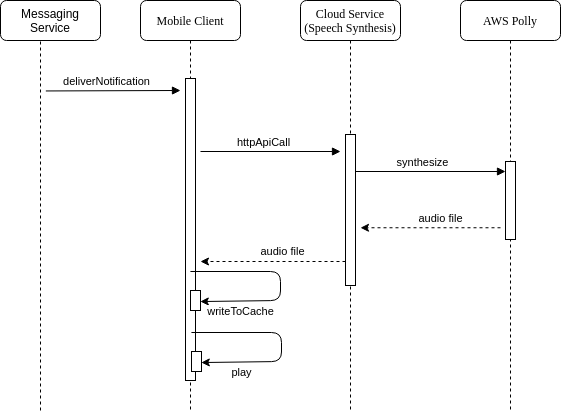
\includegraphics[width=\textwidth]{graphics/diagramms/Sequence_Speech_Synth_V01}
        \caption{Ablauf Benachrichtigung empfangen}
    \end{minipage}
\end{figure}


Anschliessend prüft, der NotificationService, ob Sprachsynthese lokal aktiviert ist.
Ist diese deaktiviert, endet die Verarbeitung.
Ist die Sprachsynthese lokal aktiviert, wird die Benachrichtigung an den SpeechSynthesisService übergeben.
Der SpeechSynthesisService prüft als erstes, ob die Sprachdaten für die empfangene Benachrichtigung bereits lokal zur Verfügung stehen.
Dies wird gemacht in dem er überprüft, ob im Applikationsverzeichnis bereits eine MP3-Datei für den Empfangenen Benachrichtigungstyp (NotificationType) in der Version der Empfangenen Benachrichtigung vorhanden ist.
Ist dies der Fall, werden die Inhalte dieser Datei abgespielt und es wird keine Anfrage an den Cloudservice versendet.
Wenn die Daten gar nicht oder nur in einer anderen Version lokal gefunden werden, wird eine Anfrage an den CloudService gesendet.
Der CloudService findet die Inhalte der relevanten Benachrichtigung in der Konfiguration und sendet eine Anfrage an den Sprachsynthese Provider.
Anschliessend leitet er die Resultate des Providers an den Client weiter.
Der Client speichert die empfangenen Daten lokal im Applikationsverzeichnis unter Id und Version des Benachrichtigungstyps (NotificationType).
Nachdem die Daten gespeichert wurden, wird deren Inhalt abgespielt.

\textbf{TODO: } Add Client View Sequence Diag


\clearpage
